% =====================================================================
% SEC 04 — Resultados
% =====================================================================
\section{Resultados}
\label{sec:resultados}

Executamos o coorte com $n\_queries=4$, orçamento $K=4$ e pool de candidatos
$N=40$ (após deduplicação por documento) sobre o corpus-piloto de 6 ângulos
$\times$ 3 documentos. Todos os valores reportados nesta seção são \emph{reais},
extraídos do relatório estruturado do \emph{benchmark}
(\texttt{benchmarks/cohort\_report.json}). Nenhum número foi interpolado ou
modificado.

\subsection{Resultados agregados por estratégia}

A Tabela~\ref{tab:resumo} apresenta as médias das métricas por estratégia ao longo
das 4 queries.

\begin{table}[ht]
\centering
\caption{Resultados agregados do coorte (médias sobre $n\_queries=4$, $K=4$).
Valores reais do \texttt{cohort\_report.json}.}
\label{tab:resumo}
\begin{tabular}{lccc}
\toprule
\textbf{Estratégia} & $\Div(\mathcal{S})$ & \emph{groundedness} & \emph{cobertura} \\
\midrule
\emph{top-k} (atual) & 0.500 & 0.4561 & 0.667 \\
MMR ($\lambda=0.7$)   & \textbf{0.750} & 0.4256 & \textbf{0.917} \\
Recamán               & 0.500 & 0.4561 & 0.667 \\
\bottomrule
\end{tabular}
\end{table}

Os resultados revelam três fatos:

\begin{figure}[ht]
\centering
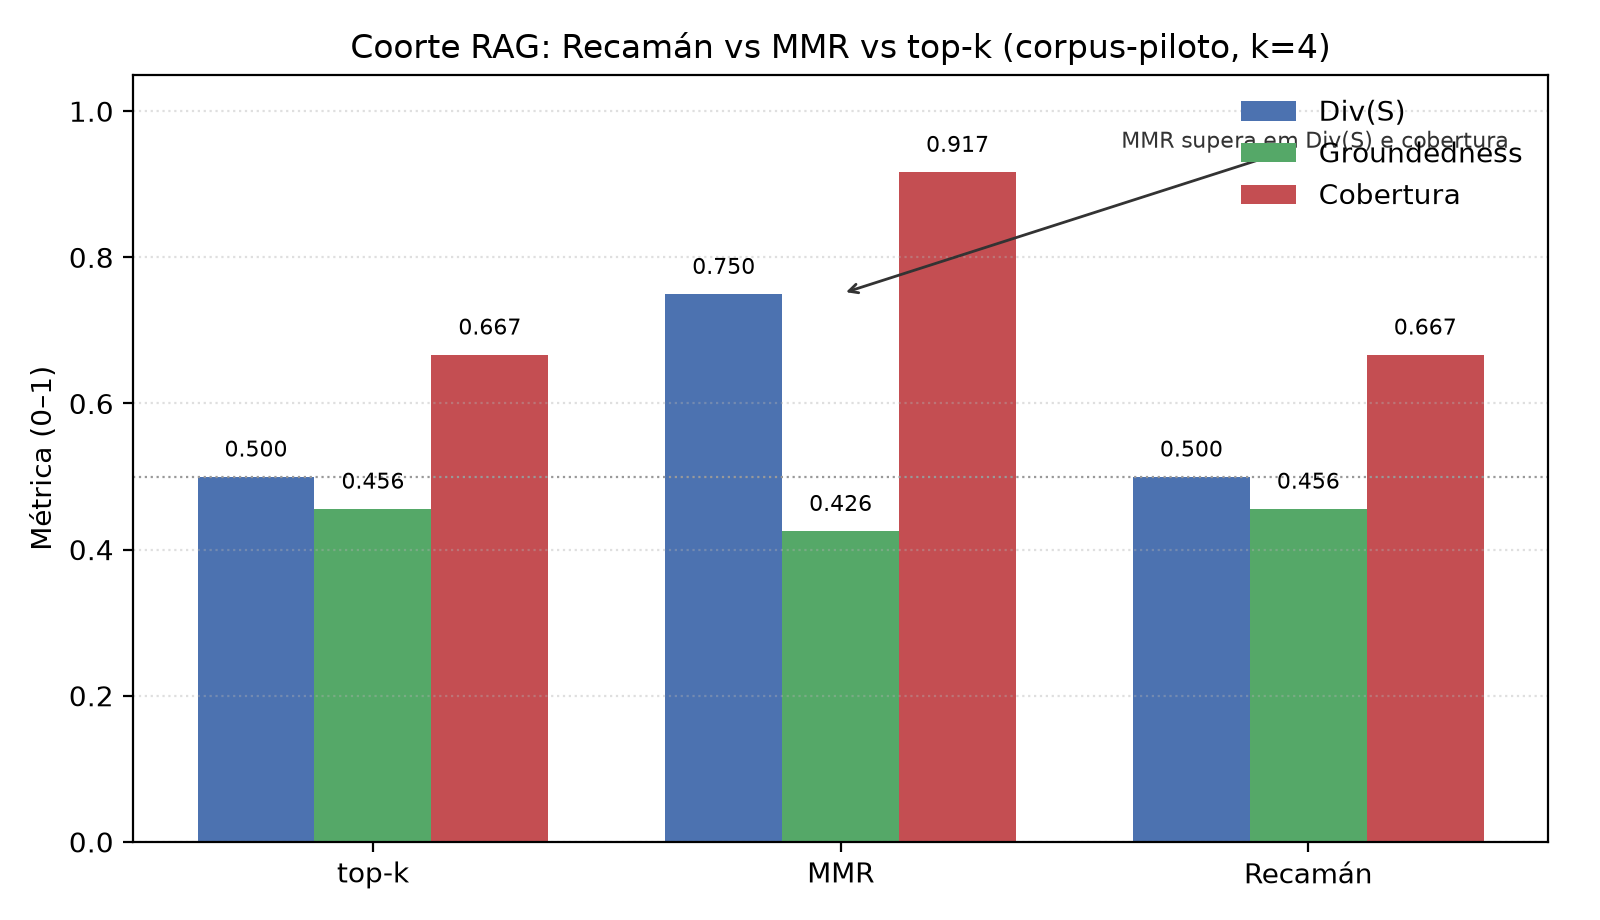
\includegraphics[width=0.85\textwidth]{figures/cohort_results.png}
\caption{Comparação das três estratégias sob diversidade, relevância e cobertura
(corpus-piloto controlado, médias sobre 4 queries). Valores iguais aos do
\texttt{cohort\_report.json}.}
\label{fig:cohort}
\end{figure}

\begin{enumerate}
  \item \textbf{Diversidade:} o MMR atinge $\Div=0{,}750$, superior ao
        \emph{top-k} ($0{,}500$) e ao Recamán ($0{,}500$). O ganho de diversidade
        do Recamán sobre o \emph{top-k} é $\Delta\Div = 0{,}0$ — um \emph{empate
        estrito}, não um ganho.
  \item \textbf{Relevância (\emph{groundedness}):} o Recamán mantém
        $\mathit{g}=0{,}4561$, idêntico ao \emph{top-k} — queda relativa $=0{,}0\%$,
        dentro da tolerância. O MMR apresenta $\mathit{g}=0{,}4256$ (queda de
        $\approx 6{,}7\%$ frente ao \emph{top-k}), acima do limiar de $5\%$
        definido.
  \item \textbf{Cobertura de ângulos:} o MMR cobre $0{,}917$ dos ângulos-alvo;
        \emph{top-k} e Recamán cobrem $0{,}667$.
\end{enumerate}

\subsection{Comportamento por query}

a Tabela~\ref{tab:porquery} detalha a diversidade por query. Observa-se que, exceto
na query 2 (em que MMR também coincide com \emph{top-k}), o MMR diverge mais em
todas as demais, enquanto Recamán permanece igual ao \emph{top-k} em todas as
queries — comportamento consistente com o achado agregado.

\begin{table}[ht]
\centering
\caption{Diversidade $\Div(\mathcal{S})$ por query.
Valores reais do \texttt{cohort\_report.json}.}
\label{tab:porquery}
\begin{tabular}{lcccc}
\toprule
\textbf{Query} & \emph{top-k} & MMR & Recamán \\
\midrule
q0 & 0.500 & 0.8333 & 0.500 \\
q1 & 0.500 & 0.8333 & 0.500 \\
q2 & 0.500 & 0.5000 & 0.500 \\
q3 & 0.500 & 0.8333 & 0.500 \\
\bottomrule
\end{tabular}
\end{table}

\subsection{Veredito da hipótese}

Com base nos critérios definidos na Seção~\ref{sec:metodo}:
\[
\underbrace{\Delta\Div(\text{Recamán}) = 0{,}0}_{\text{não estritamente }>0}
\;\Rightarrow\; \textbf{H2 refutada}
\]
Registramos, portanto, o veredito \texttt{refuta\_H2}: no corpus-piloto, a
seleção posicional por Recamán \emph{não demonstra} ganho estrito de diversidade
sobre o \emph{top-k}, enquanto o MMR demonstra ganho em 3 das 4 queries.
